\documentclass[conf]{new-aiaa}
%\documentclass[journal]{new-aiaa} for journal papers
\usepackage[utf8]{inputenc}

\usepackage{graphicx}
\usepackage{amsmath}
\usepackage[version=4]{mhchem}
\usepackage{siunitx}
\usepackage{longtable,tabularx}
\setlength\LTleft{0pt} 

\title{Interaction of Geomagnetic Storms on Earth Magnetic Anomaly Navigation}

\author{Spencer A. Freeman}
\affil{Virginia Tech, Blacksburg, VA, 24061}

\begin{document}

\maketitle

\begin{abstract}
The topic of this report is the interaction of geomagnetic storms on Earth magnetic anomaly navigation. The Earth’s magnetic field can be decomposed into subcomponents based on the source of each component. The greatest contributor is known as the core field, which is generated by the Earth's perpetually circulating molten iron core. This field is on the order of 30,000 – 50,000 nanoteslas (nT). A much smaller contributor is known as the Earth Magnetic Anomaly which is generated by induced magnetization of materials in the Earth’s crust. This field is on the order of 100’s of nT. The core field varies only over long ranges whereas the magnetic anomaly varies much greater spatially and thus provides a viable candidate signal for local navigation. Unfortunately, there are time varying components in the magnetic field that are much more difficult to predict. The ionosphere creates induced magnetic fields through the circulation of ions. This is exacerbated by solar interference which creates more ions, and thus unpredictable magnetic disturbances which corrupt the magnetic anomaly readings. This report details a study on the navigational impacts of these disturbances.
\end{abstract}

\section{Outline and Key Aspects}
\lettrine{T}{his} report is a study on the interaction of geomagnetic storms on Earth magnetic anomaly navigation. The methodology was to simulate a Kalman filter updated with simulated magnetometer measurements and observe the results under different magnetospheric conditions. Several items needed to be developed to perform the simulation.\\

\begin{enumerate}
   \item Acquire magnetic anomaly map
   \item Generate truth trajectory
   \item Develop magnetometer sensor model
        \begin{description}[font=$\bullet$\scshape\bfseries]
            \item Acquire geomagnetic storm data
            \item Implement storm data into magnetometer model
        \end{description}
   \item Create Kalman filter simulation 
       \begin{description}[font=$\bullet$\scshape\bfseries]
            \item Implement magnetometer measurement update
        \end{description}
   \item Plot and interpret results\\
\end{enumerate}

This first step was to acquire data for use in the simulation. Magnetic anomaly navigation requires a precise map of the local magnetic field which is used to relate measurements to geodetic location. Most anomaly maps are localized and do not share a common format due to their genesis in the natural resource prospecting industry. Some attempts have been made to produce global maps which combine existing data; For the purposes of this project, the National Oceanic and Atmospheric Administration (NOAA) Earth Magnetic Anomaly Grid 2-arc-minute resolution (EMAG2) v3 dataset will serve this purpose. In addition to serving as the geodetic map, EMAG2 was used to generate simulated magnetometer measurements with noise added mimicking real world data. Lastly, data representing the effects of geomagnetic storms on the magnetic field was needed. Given the randomness of their occasions, these effects are most reliably captured by persistent ground based sensors. The British Geological Survey maintains a web service called INTERMAGNET, which hosts magnetometer data recorded at dozens of sites around the world [CITE]; data from the USGS Fredericksburg, VA station was pulled for use in this project.

The key aspect of this project is studying the ability of the navigation system to handle time-varying biases in the magnetic anomaly field measurement. Since the physical sensor measures the total field strength, which is the summation of multiple components, the measurement must be processed to extract the value of the magnetic anomaly field. Geomagnetic storms induce temporary magnetic fields around the Earth which disturb the permanent magnetic field. Even given warning of solar activity, the localized effects are difficult to predict and time-varying, so accounting for the disturbances presents a challenge.

This project presents these effects by perturbing measurements of the permanent magnetic field with actual recorded data from known geomagnetic storms. In recent memory, a Coronal Mass Ejection in February 2022 produced a storm that caused global disruption including the loss of 38 commercial satellites [CITE]. The magnetic effects of this event were seen even at ground level via recording stations across the world. The data from one of these stations was used to mimic the time-varying disturbances the would likely be observed by a sensor at some location.  

\section{Background} % ==========================================

In order to motivate the study of magnetic disturbances on navigation, a review of navigation algorithms and the physics of the Earth's magnetic field is necessary. A brief, but thorough description of navigation algorithms will be presented along with the chosen architecture for this analysis. The principles of geodetic navigation are simple enough, but their practical implementation is generally quite intricate and nuanced. A simplified model will be used to analyze the topic at hand. Additionally, a review of Earth's magnetic field and the models used to describe it are presented in just enough detail to allow discussion of their use as navigation signals.

\subsection{Geodetic Navigation} % -----------------------

Navigation is the method of determining position, course, and distance traveled of some vehicle [CITE - https://www.merriam-webster.com/dictionary/navigation]. Generally defined by a global frame of reference, navigation with respect to the Earth can be considered geodetic. Some examples of this practice are global navigation satellite systems (GNSS) which use RF transmissions and precise timing to geolocate receivers. The process of navigation utilizes signals which encode information about the state of a vehicle to estimate the state or some subspace of states. Part of the process is rejection of noise, which is unavoidable in any practical navigation signal. The quintessential algorithm for state estimation is the Kalman filter, an optimal solution for filtering of noisy signals. Derivations of the Kalman filter equations are given in [CITE bar shalom]. Sparing the full derivation, the discrete-time implementation is given here. The Kalman filter is a two-step procedure:\\

\begin{enumerate}
    \item Propagate state estimate and covariance.
        \begin{description}[font=$\bullet$\scshape\bfseries]
            \item \(\overline{x} = \Phi \hat{x}\)
            \item \(\overline{P} = \Phi P \Phi^{T} + Q\)
        \end{description}
    \item Update state estimate and covariance using the measurement.
        \begin{description}[font=$\bullet$\scshape\bfseries]
            \item \(M = (M^{-1} + H^{T}R^{-1}H)^{-1}\)
            \item \(K = PH^{T}R^{-1}\)
            \item \(\hat{x} = \overline{x} + K(z - \overline{z})\) \\
        \end{description}
\end{enumerate}

The first step propagates the state estimate and state covariance given a dynamics model encoded in the state transformation matrix \(\Phi\) and process noise \(Q\). The state transformation matrix is a linearization of the system dynamics and the process noise matrix is the covariance of the noise present in the system dynamics. This term captures unmodeled or unknown dynamics and is generally used as a tuning parameter.

The second step is the measurement update. This is where measurements are processed into the state estimate and covariance. Key terms are the measurement-state transformation matrix \(H\) and the measurement covariance matrix \(R\). \(H\) is derived from the generally nonlinear formulation of the measurement as a function of the state; it is a linearization computed analytically or numerically \(H = dz/dx\). \(R\) is the measurement noise covariance and is in practice is estimated from sensor data.

\subsection{Components of Earth's Magnetic Field} % -----------------------

Magnetic fields describe the physical phenomenon of forces exerted on and generated by circulating currents and elementary particles. Magnetic fields are vector fields with magnitude and direction in 3-dimensional space and as with all vector fields, the total value at one point can be decomposed into a sum of sub components. The Earth's magnetic field is that which exists within the Earth extending to the outer magnetosphere several Earth radii outwards. There are several prime contributors to the total field which can be isolated by their source. The component buildup is given in the following equation:

\begin{equation}
    H(x, t) = H_{crust}(x) + H_{core}(x) + H_{ion}(x, t) + H_{other}(x, t), \; (nT)
\end{equation}

\(H_{core}\) is the largest magnitude component in the field. It is generated by the Earth's perpetually circulating, molten iron core which causes circulating electrical currents and thus an astronomically relevant magnetic field at the surface. It is roughly approximated by a dipole and has magnitudes on the  order of 40,000 (nT).

\(H_{ion}\) is the combination of induced magnetic fields caused by currents in the ionosphere. Solar radiation ionizes particles in the atmosphere creating a conductive plasma where electric currents can flow. These currents generate magnetic fields the superimpose onto the observed field spatially and temporally.

\(H_{other}\) is a catch all for unknown or unmodeled disturbances in the field.

\(H_{crust}\) is the component of the field which is generated by induced magnetization of conductive materials in the Earth's crust (lithosphere). This magnetization is latent from induced magnetization from existing fields becoming permanent due to cooling [CITE ]. This component varies in magnitude on the order of 100's of nanteslas and spatially in kilometers. This in conjunction with its time invariant nature (crustal magnetization varies only on geological times scales) makes it a practical candidate for map-based navigation [CITE].  

\subsection{Geomagnetic Storms} % -----------------------

Geomagnetic storms are 

\section{Data and Methods} % ==========================================

\subsection{The Kalman Filter} % -----------------------

\subsection{Magnetic Field Representation} % -----------------------

\subsection{Geomagnetic Storm Representation} % -----------------------

\begin{equation}
    H_{temporal}(x, t) = H_{crust}(x) + H_{core}(x) + H_{ion}(x, t) + H_{other}(x, t), \; (nT)
\end{equation}

\begin{equation}
    H_{ion}(x, t) = H_{temporal}(x, t) - (H_{crust}(x) + H_{core}(x) + H_{other}(x, t)), \; (nT)
\end{equation}

\section{Results} % ==========================================

\subsection{Quiet Time} % -----------------------

\subsection{Stormy} % -----------------------

\begin{figure}[h!]
\centering
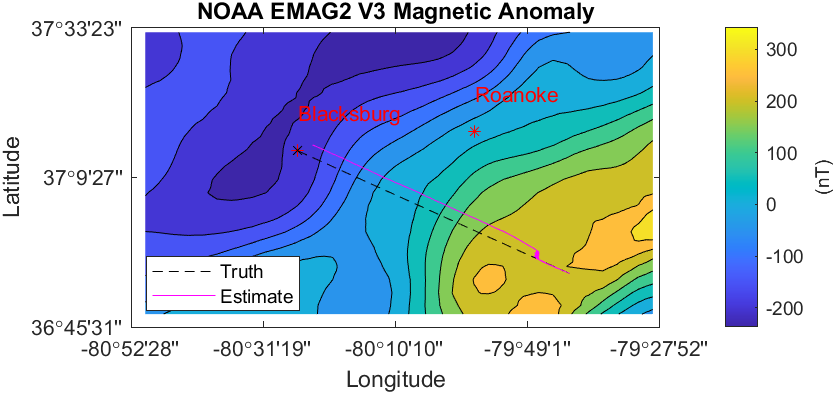
\includegraphics[width=.75\textwidth]{figures/trajectory.png}
\caption{Filter performance XXX.}
\end{figure}

\begin{figure}[h!]
\centering
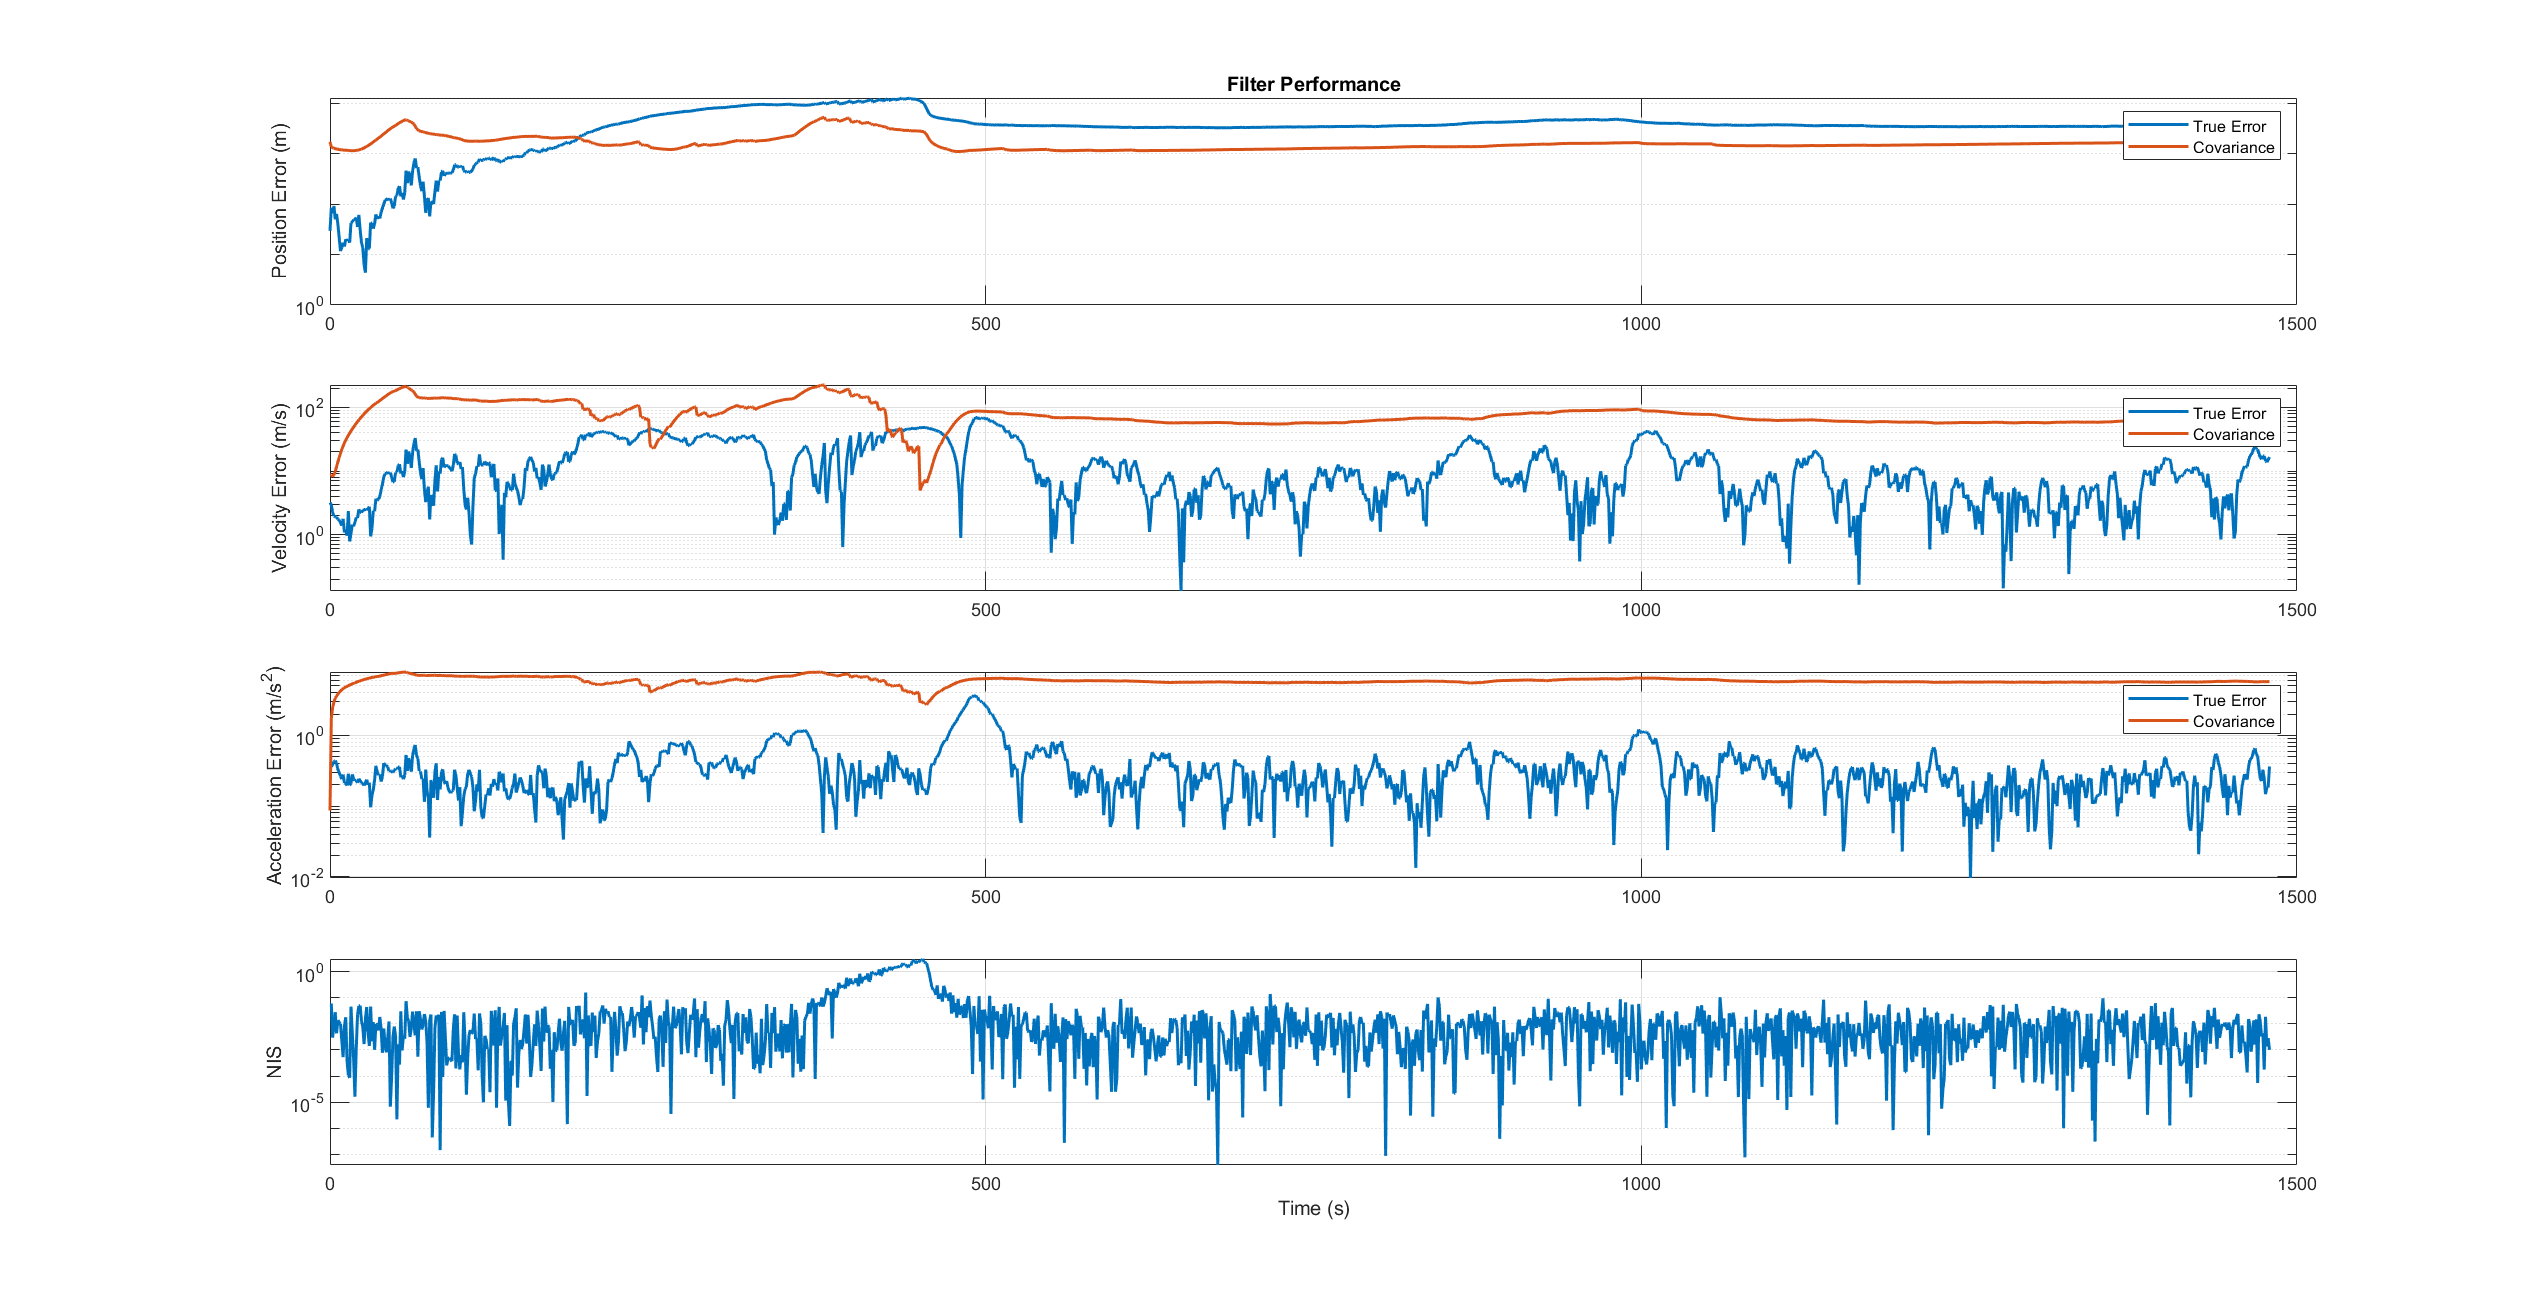
\includegraphics[width=1.0\textwidth]{figures/filter_performance.png}
\caption{Filter performance XXX.}
\end{figure}

\section{Discussion} % ==========================================

\section{Further Work} % ==========================================

\section*{Appendix} % ==========================================

\bibliography{sample} % ==========================================

\end{document}
